\chapter{Short duration conditions: diarrheal diseases}
\label{applications-short_dur}

This chapter considers the application of this framework to
conditions where the duration of disease is days or weeks. These acute
conditions, such as diarrheal disease, still fit into the
compartmental model, provided assumptions are made about the average
case duration.  The resulting estimates can be sensitive to these
assumptions, however, and just how sensitive is the topic of this
chapter.

Diarrheal diseases are a leading cause of childhood morbidity and
mortality.  Typically defined as having loose or watery stools three
or more times a day or more frequently than normal for the individual,
the diarrheal episodes typically last 1-8 days for acute cases
depending on severity. \cite{unicef_diarrhoea_2009,
  carlos_etiology_1990, lamberti_systematic_2012} Compared to many of
the other diseases discussed thus far, diarrheal diseases have a very
short duration.

Bacterial, viral and parasitic infections cause most cases of
intestinal infectious diarrhea.  Typically spread via the oral-fecal
route, water sanitation and hygiene are a large part of diarrhea
prevention.  Treatment usually involves fluid replacement, as acute
diarrhea causes fluid loss and dehydration.  Common prevention
strategies include vitamin A and zinc supplementation, vaccinations
and antibiotic regimes. \cite{wardlaw_diarrhoea:_2010,
  carlos_etiology_1990, lamberti_systematic_2012}

For the analysis of diarrheal diseases, the systematic review collected data
from surveys, hospital admissions and published studies.  The
surveys report period prevalence data whereas hospital admissions and
the majority of the literature report incidence data.  In short term
diseases, point prevalence is approximately the same as the product of
incidence and disease duration.  Therefore to avoid compositional
bias, all incidence and period prevalence estimates were converted to
point prevalence estimates using the assumption that
    \begin{equation}
    	h_{p_{point}}=h_{p_{period}} \cdot
        \frac{h_{d}}{h_{d}-1+X_{recall}}
    \end{equation}
where $h_{p_{point}}$ is the point prevalence, $X_{recall}$ is the
survey recall period and $h_{d}$ is the mean duration of the disease.
Thus the analysis includes $2029$ data points on disease prevalence
from 19 regions.  Data from the Latin America, Central region is shown
in Figure \ref{fig:app-diarrhea data}.  The prevalence data collected
in systematic review was complemented by population-level
cause-specific mortality rate estimates generated in a separate
exercise.  Since the condition is acute, the assumption that
cause-specific mortality rate is a direct measurement on $h_{p}\cdot
h_f$ is justified.  In other words, the model assumes that anyone who
died \emph{with} the disease died \emph{of} the disease.

    \begin{figure}[h]
        \begin{center}
            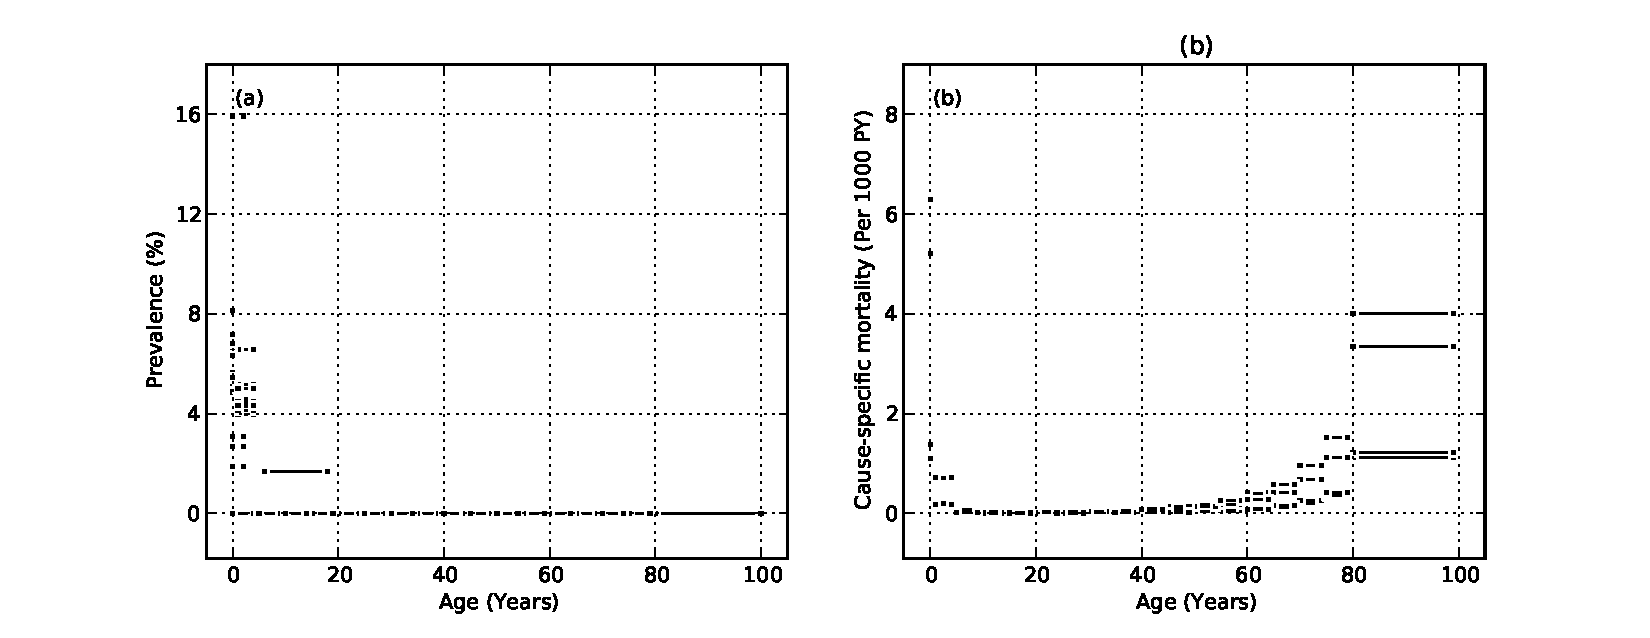
\includegraphics[width=\textwidth]{diarrhea-data.pdf}
            \caption{Diarrheal point prevalence (panel (a)) and
              cause-specific mortality (panel (b)) data in Central
              Latin America.}
            \label{fig:app-diarrhea data}
        \end{center}
    \end{figure}

Diarrheal diseases use a compartmental model to model all
epidemiological parameters for a single time, place and sex.  A
compartmental model estimates all epidemiological parameters
simultaneously which maintains internally consistent results as
discussed in Chapters \ref{sys-dynamics}.  In addition to the
systematic review data, informative priors on the duration of
diarrheal diseases help guide the modeling process.  The prior for the
length of a case is implemented as a prior on the remission hazard
$h_r$.  It is also possible to set a prior on duration directly, but
this may lead to unexpected results, since duration is affected by
remission rates and excess-mortality rates.  In a setting where the excess-mortality hazard is
small compared to the remission rate, Equation~\ref{eq:remission-duration}
approximates the relationship between duration and remission
    \begin{equation} \label{eq:remission-duration}
    	h_{r} = \frac{1}{h_{d}}
    \end{equation}
where $h_{r}$ is the epidemiological rate for remission and $h_{d}$ is
the epidemiological rate for duration in years.  Similar to the
discussion of priors in Chapter \ref{applications-con_fit_splines},
the choice of priors affects the epidemiological estimates.  However,
because the compartmental model enforces internal consistency, a
change in assumptions about the remission rate assumptions has effects
on other epidemiological parameter estimates as well, as seen in
Figure \ref{fig:app-diarrhea duration}.  Since there is no data about
disease incidence, this is the additional parameter most affected by
the change in remission rate.

    \begin{figure}[h]
        \begin{center}
            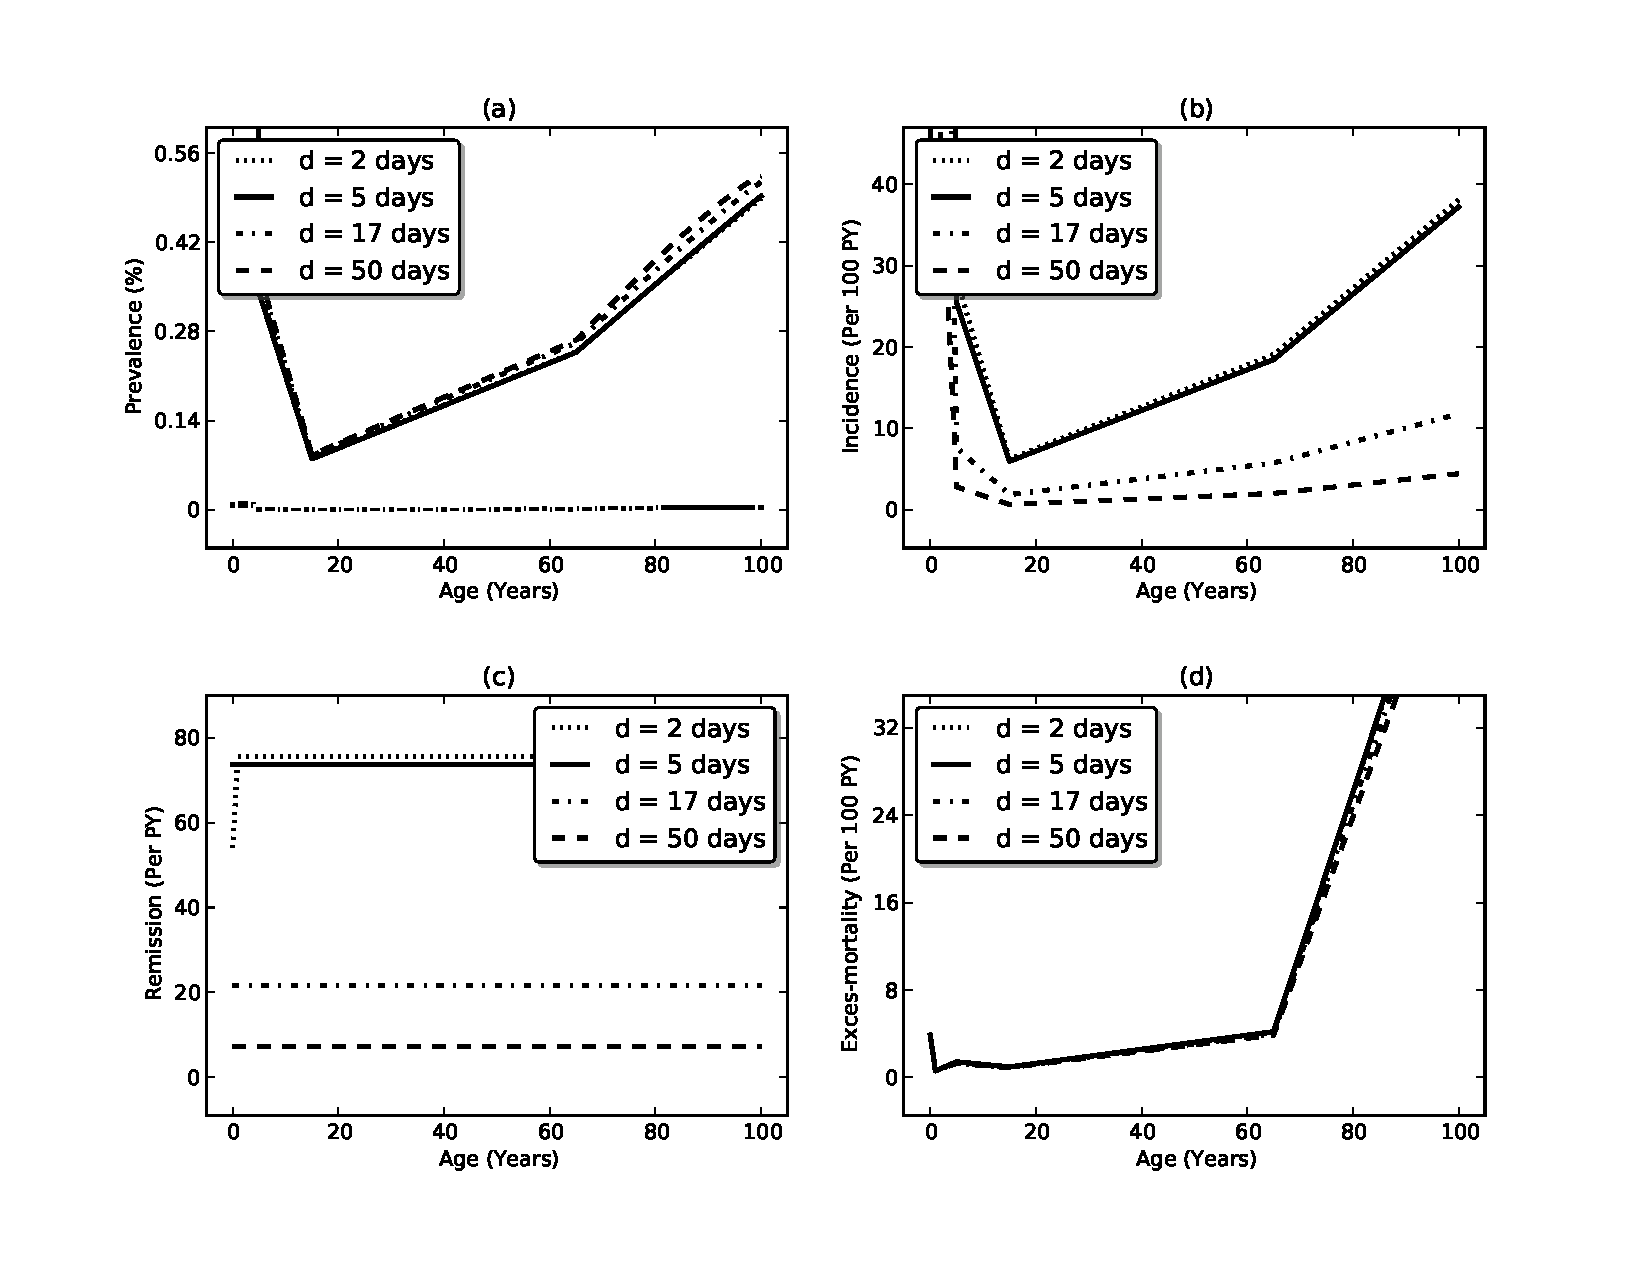
\includegraphics[width=\textwidth]{diarrhea-duration.pdf}
            \caption{Estimates of prevalence (panel (a)), incidence
              (panel (b)), remission (panel (c)) and excess-mortality
              (panel (d)) for diarrheal diseases in Central Latin
              American males in 2005 using a compartmental model with
              differing priors on disease duration, $d$.}
            \label{fig:app-diarrhea duration}
        \end{center}
    \end{figure}

TK summary and conclusion.
